
\begin{SCfigure*}
	\centering
	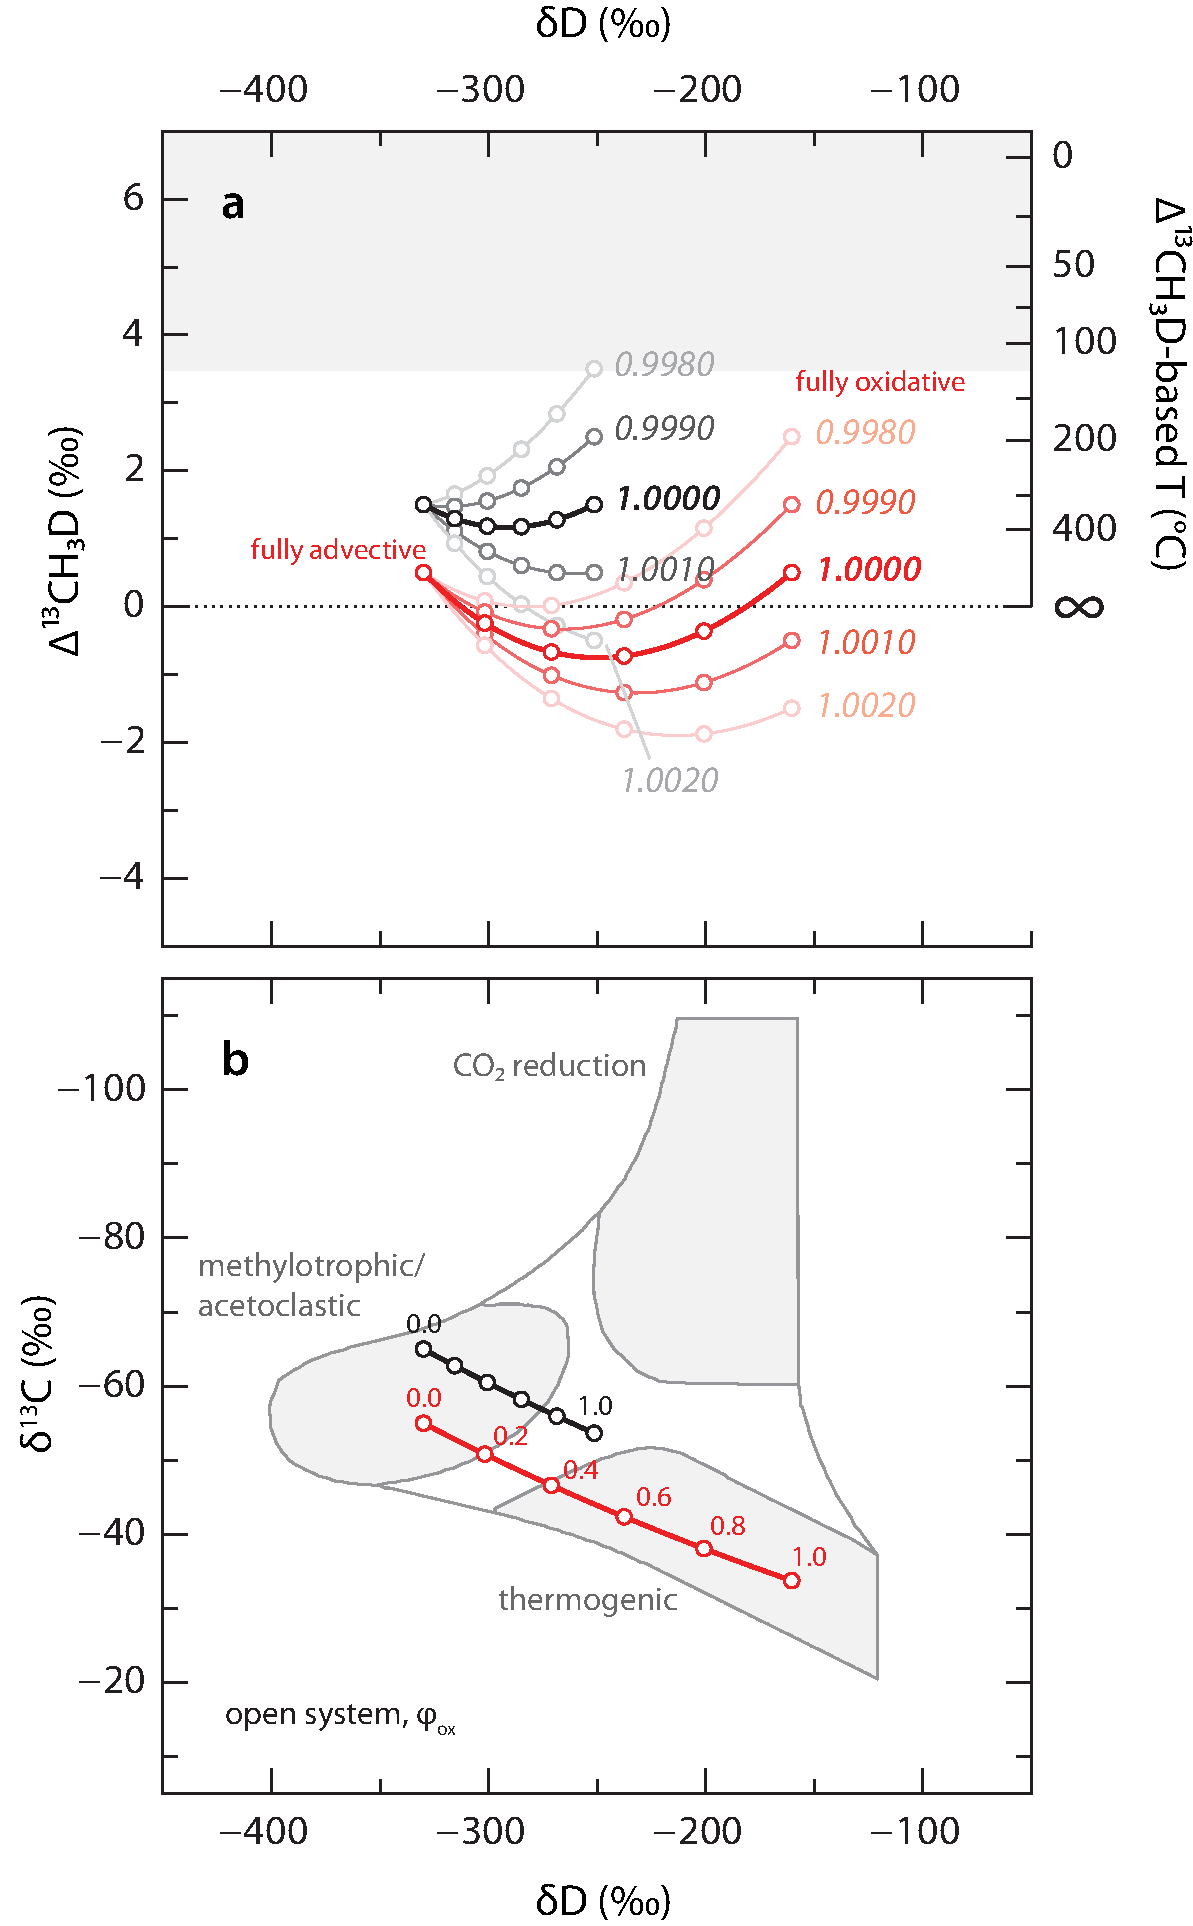
\includegraphics[width=0.5\textwidth]{figures/Fig4.5}
	\caption[Trajectories for isotope/isotopologue ratios of methane oxidized in an open system]{Modeled steady-state values of \textbf{(a)}
		Δ\textsuperscript{13}CH\textsubscript{3}D vs.\ δD and \textbf{(b)}
		δ\textsuperscript{13}C vs.\ δD of methane in an open system (\autoref{fig:4:4})
		consisting of a single source and two sinks (aerobic methane oxidation
		and advection). Advection is assumed to be non-fractionating. Lines were
		modeled using \mrefs[]{Eqns.}{eqn:4:22} and \ref{eqn:4:23}, and the same fractionation factors for
		aerobic methane oxidation as for those shown with the same line style in
		\autoref{fig:4:2}. Labels in \emph{italics} in panel (a) represent $\gamma$ values
		associated with aerobic methane oxidation. Circles are marked at
		intervals of 0.2 in $\varphi$\textsubscript{ox}, the fraction of methane removed
		via oxidation, ranging from fully advective ($\varphi$\textsubscript{ox} = 0) to
		fully oxidative ($\varphi$\textsubscript{ox} = 1), and labeled in panel (b).
		When $\varphi$\textsubscript{ox} = 0, the isotopic composition of methane in the
		reservoir is identical to that of the source. For visual clarity, the
		calculations were performed for slightly different
		δ\textsuperscript{13}C and Δ\textsuperscript{13}CH\textsubscript{3}D
		values of input methane. For description of shaded fields, see the
		caption for \autoref{fig:4:3}.}
	\label{fig:4:5}
\end{SCfigure*}